
\thispagestyle{plain}

\chapter{Konfiguration der Anwendung}\label{c_config}
Die Konfiguration der Anwendung findet hauptsächlich über die \emph{application.properties} Datei statt. Hier können sämtliche Werte wie zum Beispiel Datenbank-URL, Logging-Einstellung usw. festgelegt werden. Die Konfigurationsdateien befinden sich im Verzeichnis \emph{resources}. Siehe Listing \ref{lst:appprops} als Beispiel.

   \begin{lstlisting}[caption={application.properties},label={lst:appprops},language=Java]
app.name=weFactor

# IDENTITY (ContextIdApplicationContextInitializer)
spring.application.name=weFactor

logging.level.org.springframework.web: DEBUG
logging.level.org.hibernate: ERROR

# THYMELEAF (ThymeleafAutoConfiguration)
spring.thymeleaf.encoding=UTF-8
spring.thymeleaf.content-type=text/html


# EMBEDDED SERVER CONFIGURATION (ServerProperties)
server.tomcat.uri-encoding = UTF-8

spring.mvc.locale=en_UK
spring.mvc.date-format= dd/MM/yyyy

# INTERNATIONALIZATION (MessageSourceAutoConfiguration)
spring.messages.basename=messages
spring.messages.cacheSeconds=-1
spring.messages.encoding=UTF-8

    
   \end{lstlisting}
   Eine ausführliche Liste der Einstellmöglichkeiten ist in der Spring Dokumentation\footnote{\url{http://docs.spring.io/spring-boot/docs/current/reference/html/common-application-properties.html}} zu finden.
   
   
\section{Environments}\label{s_env}
Als Ergänzung zur \emph{application.properties} Datei können umgebungsspezifische Einstellungen festgelegt werden. Dafür muss folgende Namenskonvention eingehalten werden: \emph{application-{profile}.properties}.

So lassen sich nun unterschiedliche Datenbank-Einstellungen für die verschiedenen Zielumgebungen festlegen. Möchte man spezielle Properties für ein Profil mit dem Namen \emph{dev} anlegen, so haben sich diese in einer Datei mit dem Namen \emph{application-dev.properties} zu befinden. Profile können nun zum Beispiel über die VM-Arguments aktiviert werden (siehe Abbildung \ref{fig:active-profile}).
\begin{figure}[H]
    \centering
    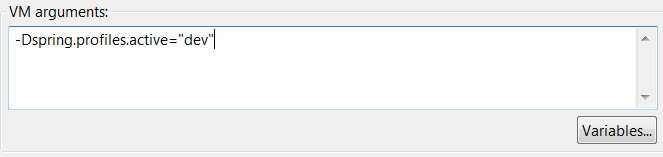
\includegraphics[width=0.8\textwidth]{Bilder/startlauncher.png}
    \caption{Profil über die VM-Arguments aktivieren}
    \label{fig:active-profile}
\end{figure}

Eine weitere Möglichkeit ist das Aktivieren eines Profils über die Annotation \emph{@ActiveProfiles}. Siehe dazu Listing \ref{lst:profileanno}.

   \begin{lstlisting}[caption={@ActiveProfiles Annotation},label={lst:profileanno},language=Java]
@ActiveProfiles("test")
public class BaseTest {...}
   \end{lstlisting}

\section{Konfiguration der Datenbank}\label{s_config_db}
Die Konfiguration der Datenbank findet ebenfalls in der Datei \emph{application.properties} statt. Siehe dazu Listing \ref{lst:dbconf} als Beispiel.
   \begin{lstlisting}[caption={Konfiguration der Datenbank},label={lst:dbconf}]
spring.datasource.url=jdbc:mysql://localhost:3306/...
spring.datasource.username=user
spring.datasource.password=secret
spring.datasource.driverClassName=com.mysql.jdbc.Driver
   \end{lstlisting}
   Sofern keine Datenbank konfiguriert ist, wird automatisch die embedded HSQLDB verwendet.


\section{Konfiguration der Social-Login-Provider}\label{s_config_social}
Zur Bereitstellung der Social-Login-Funktionalitäten wird die Bibliothek Spring-Social verwendet. Siehe dazu die Spring Dokumentation\footnote{\url{http://docs.spring.io/spring-social/docs/current/reference/htmlsingle/}}.
Die Konfiguration der Social-Login-Provider findet ebenfalls in der Datei \emph{application.properties} statt.
Siehe Listing \ref{lst:social} als Beispiel.
   \begin{lstlisting}[caption={Konfiguration der Social-Login-Provider},label={lst:social}]
# SPRING SOCIAL FACEBOOK (FacebookAutoConfiguration)
spring.social.facebook.app-id= # your application's Facebook App ID
spring.social.facebook.app-secret= # your application's Facebook App Secret

# SPRING SOCIAL LINKEDIN (LinkedInAutoConfiguration)
spring.social.linkedin.app-id= # your application's LinkedIn App ID
spring.social.linkedin.app-secret= # your application's LinkedIn App Secret

# SPRING SOCIAL TWITTER (TwitterAutoConfiguration)
spring.social.twitter.app-id= # your application's Twitter App ID
spring.social.twitter.app-secret= # your application's Twitter App Secret
   \end{lstlisting}
   
   Für die Konfiguration der Social-Provider sind zwei Einträge notwendig:
   
   \begin{itemize}
   \item app-id
   \item app-secret
   \end{itemize}
   
   Beide Werte werden von den jeweiligen Providern bereitgestellt, sobald eine entsprechende App angelegt wurde.